
\documentclass[11pt]{article}
\usepackage[utf8]{inputenc}

\usepackage{comment}
\usepackage{amsmath}
\usepackage{amsfonts}
\usepackage{amsthm}
\usepackage{mathtools}
\usepackage{amssymb}
\usepackage{verbatim}
\usepackage[shortlabels]{enumitem}
\DeclarePairedDelimiter\ceil{\lceil}{\rceil}
\DeclarePairedDelimiter\floor{\lfloor}{\rfloor}



\newcommand{\bd}{\text{bd}}
\newcommand{\cl}{\text{cl}}
\newcommand{\inte} {\text{int}}

\newcommand{\cA}{ {\cal A} }
\newcommand{\fA}{ {\mathfrak{A}} }
\newcommand{\cB}{ {\cal B} }
\newcommand{\cD}{ {\cal D} }
\newcommand{\cF}{ {\cal F} }
\newcommand{\cL}{ {\cal L} }
\newcommand{\cM}{ {\cal M} }
\newcommand{\fM}{ {\mathfrak{M}} }
\newcommand{\cN}{ {\cal N} }
\newcommand{\cP}{ {\cal P} }
\newcommand{\cV}{ {\cal V} }
\newcommand{\cW}{ {\cal W} }

\newcommand{\bC}{ {\mathbb{C}} }
\newcommand{\bN}{ {\mathbb{N}} }
\newcommand{\bQ}{ {\mathbb{Q}} }
\newcommand{\bR}{ {\mathbb{R}} }
\newcommand{\bZ}{ {\mathbb{Z}} }

\newcommand{\ba}{ \vec{a} }
\newcommand{\bb}{ \vec{b} }
\newcommand{\ve}{ \vec{e} }
\newcommand{\pp}{ \vec{p} }
\newcommand{\qq}{ \vec{q} }
\newcommand{\ts}{ \vec{s} }
\newcommand{\uu}{ \vec{u} }
\newcommand{\vv}{ \vec{v} }
\newcommand{\ww}{ \vec{w} }
\newcommand{\xx}{ \vec{x} }
\newcommand{\yy}{ \vec{y} }
\newcommand{\zz}{ \vec{z} }
\newcommand{\zv}{ \vec{0} }

\newcommand{\aks}{ ( \, \ba_k \, )_{k=1}^{\infty} }
\newcommand{\xks}{ ( \, \xx_k \, )_{k=1}^{\infty} }
\newcommand{\yks}{ ( \, \yy_k \, )_{k=1}^{\infty} }
\newcommand{\qks}{ ( q_k )_{k=1}^{\infty} }
\newcommand{\tks}{ ( t_k )_{k=1}^{\infty} }

\newcommand{\limk}{ \lim_{k \to \infty} }
\newcommand{\ee}{ \varepsilon }


\setlength{\textwidth}{6in}
\setlength{\textheight}{8.75in}
\setlength{\oddsidemargin}{.3in}
\setlength{\topmargin}{-0.1in}
\setlength{\baselineskip}{14pt}

\pagestyle{headings}

\title{Fluorescence distributions in combinatorial models of amyloid fibrils composed of split-YFP, Sup35p, and CFP}
\author{Daniel Tianming Chen \\ \texttt{dchen0@pm.me}}
%\date{June 2017}

\usepackage[numbers]{natbib}
\usepackage{graphicx}
\usepackage{url}

\begin{document}

\maketitle

\begin{abstract}
We study four combinatorial models of fluorescence in amyloid fibrils---split-YFP alone, split-YFP with Sup35p, FRET YFP/CFP, and FRET YFP/CFP with Sup35p---and show that the expected fluorescence ratio---$R_{\text{SY}}(n) := 2E(n)/n$ for split-YFP systems, $R_{\text{F}}(n) := E(n)/n$ for FRET---converges to $2/3$, $1/3$, $1/2$, and $2/9$ respectively as the amyloid length $n \to \infty$. For split-YFP systems, we derive exact probability distributions $P(n,k)$ via generating functions applied to constrained binary strings, obtaining closed-form evaluations of $k \cdot 2^k$-weighted sums along the shallow diagonals of Pascal's triangle---identities related to known sequences (OEIS A127976, A095977) but arising here in a new biophysical context. The same bivariate generating-function framework, applied via two-state transfer matrices, unifies Sections 3 and 5: in each case the joint distribution $P(n, k)$ is encoded by a rational generating function of the form $(1 + \alpha(w) z)/(1 - \beta(w) z - \gamma(w) z^2)$, from which expected values and variances follow by differentiation at $w = 1$. These results are independently verified by Markov chain arguments and (in the unequal-concentration setting) by Monte Carlo spot checks. For FRET systems, the absence of a blocking constraint also permits a direct linearity-of-expectation computation, including an expected-value extension to a finite interaction radius $r$. All expectation and variance formulas are exact for finite $n$, not merely asymptotic.
\end{abstract}

\section{Introduction}
\textit{Amyloids} are fibrillar protein aggregates characterized by their distinctive $\beta$-sheet structure, where proteins self-assemble into highly ordered stacks \cite{chiti2006}. For the purposes of our mathematical analysis, we can abstract these complex biochemical structures into a simplified model where individual proteins, denoted as A,B,C,..., form sequential patterns in their stacking arrangements (e.g., ABBACCBCBCA...). This abstraction, while preserving the essential features of protein ordering within amyloid fibrils, transforms a complex biophysical system into a tractable mathematical framework. Our combinatorial approach follows the general framework of analytic combinatorics \cite[Ch.~I]{flajolet2009}. By viewing amyloid assembly through this lens, we can leverage classical combinatorial enumeration methods to analyze their structural properties, providing insights into both their formation patterns and potential biological implications. In particular, we study amyloids of different compositions, firstly just Split Yellow Fluorescent Proteins (split-YFP), a technique based on bimolecular fluorescence complementation \cite{hu2002}, then split-YFPs and Saccharomyces cerevisiae eukaryotic translation release factor Sup35p, and finally split-YFP and Sup35p under F\"{o}rster resonance energy transfer (FRET) \cite{forster1948} lighting. A specific quantity of interest is the expected number of \textit{fluorescing locations}---points between two adjacent proteins in the amyloid stack at which a fluorescent interaction occurs (a fusion in the split-YFP settings, a $\{C, Y\}$ adjacency in the FRET settings). We derive the full probability distributions $P(n,k)$ for the number of fluorescing sites and closed-form expressions for the expected values using combinatorial generating functions, Markov chains, and regular expressions. In the split-YFP settings, the adjacency blocking constraint leads to nontrivial combinatorial identities involving sums such as $\sum_{k=1}^{\floor{n/2}} k\, 2^k \binom{n-k}{k}$, which we evaluate via generating function techniques \cite{wilf2006}. Two independent derivations---direct summation and Markov chain arguments---yield the same closed forms, providing mutual verification. The limiting fluorescence ratios are $2/3$, $1/3$, $1/2$, and $2/9$ for the four protein systems studied. The closed-form identities that arise turn out to match known OEIS sequences (A127976, A095977); the contribution of this work is not the identities themselves, but the combinatorial pipeline connecting a biophysical model to these sequences, providing a new interpretation in terms of fluorescence statistics. Several modeling assumptions should be stated at the outset. First, we assume that proteins are independently and uniformly distributed in the amyloid sequence. Real amyloid assembly is templated and cooperative \cite{chiti2006}, so this i.i.d.\ assumption constitutes a \textit{combinatorial null model}---a baseline against which non-random assembly effects could be detected, rather than a mechanistic description of fibril growth. Second, in the split-YFP sections, we model fluorophore reconstitution as a purely combinatorial adjacency event; we do not capture the irreversible, thermodynamically driven nature of bimolecular fluorescence complementation \cite{hu2002}. Third, in the FRET sections, we initially restrict interactions to nearest neighbors in the fibril, then record the expected-value extension to a finite interaction radius in Section~\ref{sec:variance-radius}. In practice, the inter-strand spacing in cross-$\beta$ amyloid structure is approximately 0.47\,nm, while the F\"{o}rster radius for the CFP--YFP pair is approximately 4.9\,nm \cite{forster1948, lakowicz2006}, so FRET can occur across roughly ten subunits. The nearest-neighbor restriction is therefore a significant simplification adopted for analytical tractability; extending the full distribution to a larger interaction radius would change the combinatorial structure. Finally, the equal-concentration assumption ($p = 1/2$ or $1/3$ per protein type) is adopted throughout; we discuss the generalization to unequal concentrations in Section~\ref{sec:unequal}.

\section{Analysis of exclusively split-YFP Amyloids}
Let us first analyze amyloids consisting solely of YFP. YFP is a single polypeptide chain that can be split into two fragments, referred to as split-YFP. Call the distinct halves A and B. It is when these two halves A and B fuse that fluorescence occurs at the point of contact. There are no restrictions on the patterns in the amyloid - one can view all combinations of such halves via the regular expression $\{A,B\}^*$. 

We are interested in positions of an amyloid where A and B come together and fuse, producing yellow fluorescence. Such a scenario is essentially the reconstitution of the full fluorophore structure of YFP. We refer to such points in the amyloid stack as \textit{fluorescing locations} (or \textit{fluorescing sites}) throughout this paper. The same terminology applies in Sections~\ref{sec:fret}--\ref{sec:fret-sup35} to the FRET settings, where a fluorescing location is a $\{C, Y\}$ adjacency at which energy transfer occurs.

Let $n$ be the number of split-YFPs in a given amyloid. Clearly, there are $2^n$ possible amyloids of length $n$.

We will start with the case where the halves of Split-YFP are well-mixed in a neutral solution and of equal concentrations, and are thus equally likely to appear as the next protein in an amyloid sequence. 

\subsection{Lighting Patterns and 01 representations}

We abstract away from A and B specifically and instead analyze the ``lighting patterns'' of amyloids of length $n$, defined as follows.

We ask: How many distinct patterns of fluorescing locations could we possibly see from an amyloid of length n?

We define the \textit{01 representation} (or \textit{01 pattern}) of an amyloid $s_1 s_2 \cdots s_n \in \{A,B\}^n$ as the binary string $f_1 f_2 \cdots f_n \in \{0,1\}^n$ given by:
\[
f_i = \begin{cases}
0, & \text{if } i = 1, \\
1, & \text{if } i \ge 2,\ s_i \neq s_{i-1}, \text{ and } f_{i-1} = 0, \\
0, & \text{otherwise.}
\end{cases}
\]
Informally, $f_i = 1$ indicates that a fusion occurs between positions $i-1$ and $i$, attributed to the later index $i$: the protein $s_i$ differs from its neighbor $s_{i-1}$ and that neighbor was not already consumed by a prior fusion. The first protein always receives $f_1 = 0$ since there is no predecessor. The blocking constraint ($f_{i-1} = 0$ required) ensures that both proteins in a fused pair are ``used up,'' preventing cascading fusions. Note that the 01 representation has the same length as the amyloid, and the mapping $f$ is well-defined for any sequence in $\{A,B\}^n$.

The left-to-right, greedy pairing rule reflects the sequential nature of amyloid polymerization: proteins are incorporated one at a time at the growing end of the fibril, and each newly added protein either fuses with the current endpoint or does not. This greedy convention is motivated by the kinetics of sequential assembly---once a split-YFP pair reconstitutes, the resulting fluorophore is thermodynamically stable and irreversible \cite{hu2002}, so later arrivals cannot displace it.

For example, if we have ABBAAAAABA, then reading from left to right (because we have to think about how these proteins were added one at a time to analyze which ones fused), we get the 01 representation 0101000010. Writing these two representations side by side shows it:

\begin{alignat*}{10}
&A &B &B &A &A &A &A &A &B &A \\
&0 &1 &0 &1 &0 &0 &0 &0 &1 &0
\end{alignat*}


We always start with a 0, since the first protein cannot cause the (non-existent) previous protein to fluoresce. Doing this, we no longer need think about whether we started with an A or a B.

As another example,

\begin{alignat*}{34}
&B &B &B &B &A &B &A &B &A &B &A &B &A &B &A &B &A &B &A &A &A &A &B &A &A &B &A &B &B &B &B &A &B &A  \\
&0 &0 &0 &0 &1 &0 &1 &0 &1 &0 &1 &0 &1 &0 &1 &0 &1 &0 &1  &0 &0 &0 &1 &0 &0 &1 &0 &1 &0 &0 &0 &1 &0 &1
\end{alignat*} 
We observe that an unambiguous regular expression for these 01 patterns is $(0^*01)^* 0^*$ (non-ambiguous in the sense required by the symbolic method: each string has a unique parse). Note that if we were looking at an amyloid without knowing what the proteins actually were, we would still be able to identify its 01 pattern by looking at the fluorescing locations. Indeed, each fluorescing location corresponds to a 1.

We can count the total number of distinct 01 patterns of length $n$ using the symbolic method for regular expressions \cite[\S I.4]{flajolet2009}. Note that $(0^*01)^* 0^* = (0^+1)^* 0^*$: each block $0^*01$ consists of zero or more leading zeros followed by $01$, so the trailing $0$ of $0^*$ and the leading $0$ of $01$ merge to give at least one zero before the $1$, hence $0^*01 = 0^+1$. We assign weight $x$ per symbol. Each block $0^*01 = 0^+1$ has generating function $\frac{x}{1-x} \cdot x = \frac{x^2}{1-x}$, and the Kleene star $(0^*01)^*$ has generating function $\frac{1}{1 - x^2/(1-x)} = \frac{1-x}{1-x-x^2}$. Including the trailing $0^*$ with generating function $\frac{1}{1-x}$, we obtain:
\[
G(x) := \sum_{n=0}^\infty a_n x^n = \frac{1-x}{1-x-x^2} \cdot \frac{1}{1-x} = \frac{1}{1-x-x^2}
\]

Since $(1-x-x^2)\sum_{n \ge 0} a_n x^n = 1$, we read off the recurrence $a_n = a_{n-1} + a_{n-2}$ for $n \ge 2$, with $a_0 = a_1 = 1$.

We see that $a_0 = 1$, $a_1 = 1$, $a_2 = 2$, $a_3 = 3$, $a_4 = 5$, $a_5 = 8$, etc.

So $a_n = F_{n+1}$, where $F_n$ is the Fibonacci sequence with the standard convention $F_1 = F_2 = 1$. The coefficients $\binom{n-k}{k}$ appearing in this sum are precisely the entries along the \textit{shallow diagonals} of Pascal's triangle, and the identity $a_n = F_{n+1}$ is a well-known consequence of summing along these diagonals. The weighted sums $S_1(n)$ and $S_2(n)$ evaluated in Section 2.4 can be viewed as weighted sums along these same diagonals, with each entry scaled by $k \cdot 2^k$.

\subsection{Probability of $k$ fluorescing locations in length $n$ amyloid }

We now analyze the probability of seeing $k$ fluorescing locations in an amyloid of length $n$.

%This is equivalent to the probability of observing an amyloid of length $n$ with $k$ 1's in its 01 pattern.

\subsubsection{Distinct 01 patterns with $k$ 1s}
First, let us count the number of 01 patterns of length $n$ with $k$ 1s. Our invariant states that no 1s may be adjacent, and the first digit must be a zero. Since $f_1 = 0$ always, the $k$ ones must be placed among positions $2, 3, \ldots, n$ (i.e., $n - 1$ available positions) with no two adjacent. This is equivalent to placing $k$ non-adjacent objects in $n - 1$ boxes, giving:
\[
N(n,k) := \binom{n-k}{k}, \quad k \leq \floor{n/2}
\]
Indeed, the number of ways to place $k$ non-adjacent objects in $m$ boxes is $\binom{m-k+1}{k}$ (see \cite[Exercise~1.34]{stanley2012}); setting $m = n - 1$ gives $\binom{n-k}{k}$ as claimed.


\subsubsection{Distinct amyloids with $k$ 1s}
Now, for $k \ge 1$, the number of distinct amyloids of length $n$ with $k$ fluorescing pairs is:
\[
    \cA(n,k) = 2^k \cdot N(n-2,k-1) + 2^{k+1}  \cdot N(n-1,k) = 2^k \binom{n-k-1}{k-1} + 2^{k+1} \binom{n-k-1}{k}
\]
The zero-fluorescence case is $\cA(n,0) = 2$, corresponding to the two constant amyloids $AA\cdots A$ and $BB\cdots B$.
Throughout, binomial coefficients with lower index outside the usual range are interpreted as zero; nevertheless the displayed formula for $\cA(n,k)$ is stated for $k \ge 1$, with $k=0$ handled separately.

To justify the formula, fix an admissible 01 pattern $f$ with $k$ ones. Once $s_1$ is chosen, every later protein is determined except immediately after a $1$ in the 01 pattern: if $f_i=1$, then $s_i$ is forced to be the opposite of $s_{i-1}$; if $f_i=0$ and $f_{i-1}=0$, then $s_i$ is forced to equal $s_{i-1}$; if $f_i=0$ and $f_{i-1}=1$, then $s_i$ is free because the previous protein has already been consumed by a fusion. Thus a fixed pattern ending in $0$ has $2^{k+1}$ realizing amyloids (the initial choice, plus one free choice after each of the $k$ ones), while a fixed pattern ending in $1$ has $2^k$ realizing amyloids.

It remains only to count admissible 01 patterns by their final digit. Patterns ending in $0$ are obtained by appending a zero to a length-$(n-1)$ admissible pattern with $k$ ones, giving $N(n-1,k)$ choices. Patterns ending in $1$ must have $f_{n-1}=0$, and deleting the final $01$ leaves a length-$(n-2)$ admissible pattern with $k-1$ ones, giving $N(n-2,k-1)$ choices. Multiplying by the fixed-pattern counts proves the displayed formula.

For example, when $k = 5$ the two cases have the following degrees of freedom:

\textbf{01 pattern ends with a 0}

Consider the following pattern. We write the number of possible proteins (A or B) at that location below the corresponding location of the pattern.
\begin{align*} 
    & 000010000101001000010000 \\
    & 211112111121211211112111
\end{align*}
Indeed, for each block of 0's, at the beginning of the block, any of either A or B may appear there, since it will not fuse with the previous protein. Then thereafter each protein is uniquely determined by this choice through to the 1 that appears.

Any pattern of this case therefore has $2^{k+1}$ possible amyloids associated with it. There are $N(n-1,k)$ possible patterns for this case. 

\textbf{01 pattern ends with a 1}

Consider the following 01 pattern. We write the number of possible proteins (A or B) at that location below the corresponding location of the 01 pattern.
\begin{align*} 
    & 000010000101001000000001 \\
    & 211112111121211211111111
\end{align*}

As we can see, putting a 1 at the end of the 01 pattern implies only $2^k$ possible amyloids with the particular pattern. There are $N(n-2, k - 1)$ patterns with this property.

\textbf{Verification.} For $n = 4$, $k = 1$: $\cA(4,1) = 2^1 \binom{2}{0} + 2^2 \binom{2}{1} = 2 + 8 = 10$. For $k = 2$: $\cA(4,2) = 2^2 \binom{1}{1} + 2^3 \binom{1}{2} = 4 + 0 = 4$ (the only 01 pattern is $0101$, giving amyloids ABAB, BABA, ABBA, BAAB). With $\cA(4,0) = 2$ (AAAA and BBBB), we have $2 + 10 + 4 = 16 = 2^4$. $\checkmark$

Hence the probability of seeing $k$ fluorescing pairs in an amyloid of length $n$ is

\[
P(n,k) = \frac{\cA(n,k)}{2^n}
\]

\subsection{Expected number of fluorescing locations}

This is simply the sum:

\[
    E(n) = \frac{1}{2^n}\sum_{k=1}^{\floor{n/2}} k \cdot \cA(n,k) = \frac{1}{2^n}\sum_{k=1}^{\floor{n/2}} k \left( 2^k \binom{n-k-1}{k-1} + 2^{k+1} \binom{n-k-1}{k} \right)
\]

by definition of expected value.

\subsection{Expected percentage of proteins involved in fluorescence}

Since each fluorescing location involves two proteins, the fraction of proteins participating in fluorescence is:

\[
    R_{\text{SY}}(n) := \frac{2E(n)}{n} = \frac{1}{n \cdot 2^{n-1}}\sum_{k=1}^{\floor{n/2}} k \left( 2^k \binom{n-k-1}{k-1} + 2^{k+1} \binom{n-k-1}{k} \right)
\]

We claim that
\begin{equation}\label{eq:sum1}
\sum_{k=1}^{\floor{n/2}} k 2^k \binom{n-k-1}{k-1} = \frac{2^n (3n+2) + 2(6n-1)(-1)^n}{27}
\end{equation}

and

\begin{equation}\label{eq:sum2}
\sum_{k=1}^{\floor{n/2}} k 2^k \binom{n-k-1}{k} = \frac{2^n (3n-4)-2(3n-2)(-1)^n}{27}
\end{equation}

We prove both identities using ordinary generating functions.

We will use the identity (see, e.g., \cite[\S 1.2]{wilf2006}) that for any fixed $j \ge 0$,
\begin{equation}\label{eq:binom-ogf}
\sum_{n \ge 2j} \binom{n-j}{j} x^n = \frac{x^{2j}}{(1-x)^{j+1}}
\end{equation}
which follows from the substitution $m = n - j$ and the known generating function
\[
\sum_{m \ge j} \binom{m}{j} x^m = \frac{x^j}{(1-x)^{j+1}}.
\]

\textbf{Proof of (\ref{eq:sum1}).} Let $S_1(n) := \sum_{k=1}^{\floor{n/2}} k\, 2^k \binom{n-k-1}{k-1}$. We derive the ordinary generating function $G_1(x) = \sum_{n \ge 0} S_1(n) x^n$.

Using the substitution $j = k - 1$,
\[
S_1(n) = \sum_{j \ge 0} (j+1)\, 2^{j+1} \binom{n - j - 2}{j}
\]
Working as a formal power series, we may interchange the order of summation termwise. Applying (\ref{eq:binom-ogf}) with a shift $n \mapsto n - 2$:
\[
G_1(x) = \sum_{j \ge 0}(j+1)\, 2^{j+1} \cdot \frac{x^{2j+2}}{(1-x)^{j+1}}
= \frac{2x^2}{1-x} \sum_{j \ge 0} (j+1) \left( \frac{2x^2}{1-x} \right)^j
\]
Setting $u = 2x^2/(1-x)$ and using $\sum_{j \ge 0}(j+1) u^j = 1/(1-u)^2$, we have
\[
G_1(x) = \frac{2x^2}{1-x} \cdot \frac{1}{(1-u)^2}
\]
Since $1 - u = (1 - x - 2x^2)/(1-x) = (1-2x)(1+x)/(1-x)$, this simplifies to
\[
G_1(x) = \frac{2x^2(1-x)}{(1-2x)^2(1+x)^2}
\]
We now perform a partial fraction decomposition:
\[
G_1(x) = \frac{\alpha}{1-2x} + \frac{\beta}{(1-2x)^2} + \frac{\gamma}{1+x} + \frac{\delta}{(1+x)^2}
\]
Multiplying both sides by $(1-2x)^2(1+x)^2$ and evaluating at $x = 1/2$ gives $\beta = 1/9$, and at $x = -1$ gives $\delta = 4/9$. Expanding the right-hand side and comparing coefficients of $x^0$ and $x^1$ then yields $\alpha = -1/27$ and $\gamma = -14/27$. Now, using the standard power series
\begin{align*}
\frac{1}{1-2x} &= \sum_{n \ge 0} 2^n x^n, &
\frac{1}{(1-2x)^2} &= \sum_{n \ge 0} (n+1)\, 2^n x^n \\
\frac{1}{1+x} &= \sum_{n \ge 0} (-1)^n x^n, &
\frac{1}{(1+x)^2} &= \sum_{n \ge 0} (n+1)(-1)^n x^n
\end{align*}
we extract the coefficient of $x^n$:
\begin{align*}
S_1(n) &= -\frac{1}{27} \cdot 2^n + \frac{1}{9}(n+1)\, 2^n - \frac{14}{27}(-1)^n + \frac{4}{9}(n+1)(-1)^n \\
&= \frac{1}{27}\left[ 2^n(-1 + 3n + 3) + (-1)^n(-14 + 12n + 12) \right] \\
&= \frac{2^n(3n+2) + 2(6n-1)(-1)^n}{27}
\end{align*}
as claimed. $\square$

\textbf{Proof of (\ref{eq:sum2}).} Let $S_2(n) := \sum_{k=1}^{\floor{n/2}} k\, 2^k \binom{n-k-1}{k}$. As before, applying (\ref{eq:binom-ogf}):
\[
G_2(x) = \sum_{n \ge 0} S_2(n) x^n = \sum_{k \ge 1} k \cdot 2^k \cdot \frac{x^{2k+1}}{(1-x)^{k+1}} = \frac{x}{1-x} \cdot \frac{u}{(1-u)^2}
\]
where $u = 2x^2/(1-x)$ as before. This simplifies to
\[
G_2(x) = \frac{2x^3}{(1-2x)^2(1+x)^2}
\]
Performing partial fractions, evaluating at $x = 1/2$ gives $\beta = 1/9$ and at $x = -1$ gives $\delta = -2/9$. Comparing coefficients of $x^0$ and $x^1$ yields $\alpha = -7/27$ and $\gamma = 10/27$. Extracting coefficients:
\begin{align*}
S_2(n) &= -\frac{7}{27}\cdot 2^n + \frac{1}{9}(n+1)\,2^n + \frac{10}{27}(-1)^n - \frac{2}{9}(n+1)(-1)^n \\
&= \frac{1}{27}\left[2^n(-7+3n+3) + (-1)^n(10-6n-6)\right] \\
&= \frac{2^n(3n-4) - 2(3n-2)(-1)^n}{27}
\end{align*}
as claimed. $\square$

Substituting (\ref{eq:sum1}) and (\ref{eq:sum2}):

\begin{align}
 R_{\text{SY}}(n) &= \frac{1}{n \cdot 2^{n-1}}\sum_{k=1}^{\floor{n/2}} k \left( 2^k \binom{n-k-1}{k-1} + 2^{k+1} \binom{n-k-1}{k} \right) \\
 &= \frac{1}{n \cdot 2^{n-1}} \left(\frac{2^n (3n+2) + 2(6n-1)(-1)^n}{27}  + 2 \cdot \frac{2^n (3n-4)-2(3n-2)(-1)^n}{27} \right) \\
 &= \frac{1}{n \cdot 2^{n-1}} \cdot \frac{2^n(9n-6) + 6(-1)^n}{27} \\
 &= \frac{2(9n-6)}{27n} + \frac{6(-1)^n}{27n \cdot 2^{n-1}} \\
 &= \frac{2(3n-2)}{9n} + \frac{2(-1)^n}{9n \cdot 2^{n-1}}
\end{align}

Then as $n \rightarrow \infty$, the second term vanishes and we have

\begin{align}
    \lim_{n \rightarrow \infty} R_{\text{SY}}(n) &= \lim_{n \rightarrow \infty} \frac{2(3n-2)}{9n} = \frac{6}{9} = \frac{2}{3}
\end{align}

\subsubsection{Weighted shallow diagonal identities}

The identities (\ref{eq:sum1}) and (\ref{eq:sum2}) have a natural interpretation in terms of Pascal's triangle. Recall that the entries along the shallow diagonals of Pascal's triangle are $\binom{n-k}{k}$ for $k = 0, 1, \ldots, \floor{n/2}$, and their sum $\sum_{k=0}^{\floor{n/2}} \binom{n-k}{k} = F_{n+1}$ yields the Fibonacci numbers (Section 2.1). The identities (\ref{eq:sum1}) and (\ref{eq:sum2}) provide closed-form evaluations of \textit{weighted} sums along these same diagonals, where each entry is scaled by $k \cdot 2^k$:
\begin{align}
\sum_{k=1}^{\floor{n/2}} k \cdot 2^k \binom{n-k-1}{k-1} &= \frac{2^n(3n+2) + 2(6n-1)(-1)^n}{27} \label{eq:diag1} \\[6pt]
\sum_{k=1}^{\floor{n/2}} k \cdot 2^k \binom{n-k-1}{k} &= \frac{2^n(3n-4) - 2(3n-2)(-1)^n}{27} \label{eq:diag2}
\end{align}
These identities arise here from the fluorescence analysis, but the sequences themselves are not new. Specifically, $S_1(n) = 2 \cdot \text{A127976}(n-1)$ and $S_2(n) = \text{A095977}(n-2)$, where A127976 arises as a convolution of Jacobsthal numbers and A095977 counts $2 \times 2$ tiles in tilings of $3 \times (n+1)$ rectangles. Both sequences satisfy the linear recurrence $a_n = 2a_{n-1} + 3a_{n-2} - 4a_{n-3} - 4a_{n-4}$ with different initial conditions, which can be verified from the generating function denominator $(1+x)^2(1-2x)^2 = 1 - 2x - 3x^2 + 4x^3 + 4x^4$. Direct computation confirms: $S_1(2) = 2 = 2 \cdot \text{A127976}(1)$ and $S_2(3) = 2 = \text{A095977}(1)$, with subsequent values matching by the shared recurrence.

The fact that the same sequences govern such disparate problems---protein fluorescence in amyloid fibrils, convolutions of Jacobsthal numbers, and rectangle tilings---reflects a deeper structural phenomenon: all three settings reduce to constrained binary strings enumerated by the same rational generating functions with denominator $(1+x)^2(1-2x)^2$. The contribution of the present work is not the identities themselves, but the combinatorial pipeline that connects the biophysical model (protein sequences $\to$ constrained 01 patterns $\to$ generating functions) to these known sequences, providing a new interpretation in terms of fluorescence statistics.

As a corollary, the linear combination $S_1(n) + 2\,S_2(n) = \bigl[2^n(9n-6) + 6(-1)^n\bigr]/27$ governs the expected fluorescence in split-YFP amyloids, connecting these combinatorial identities directly to the biophysical application.

\subsubsection{Alternative derivation via Markov chain}

We can also derive $E(n)$ directly by a Markov chain argument \cite{norris1997}, bypassing $\cA(n,k)$ entirely. Consider building an amyloid one protein at a time, where each protein is independently A or B with equal probability $1/2$. Define two states based on the rightmost protein:
\begin{itemize}
\item \textbf{State $p$}: the rightmost protein is \textit{not} part of a fused pair.
\item \textbf{State $q$}: the rightmost protein is part of a fused pair.
\end{itemize}

From state $p$ (say the rightmost protein is A, unfused): with probability $1/2$ the next protein is A (same type, no fusion, stay in $p$), and with probability $1/2$ it is B (fusion, go to $q$, $+1$ fluorescence). By symmetry, the case for B is identical. So from $p$: transition to $p$ with probability $1/2$ and to $q$ with probability $1/2$, with expected fluorescence $1/2$.

From state $q$ (rightmost protein is fused): the next protein is A or B each with probability $1/2$, and in either case goes to state $p$ with no fluorescence (since the current protein is already fused). So from $q$: transition to $p$ with probability $1$.

With $p_1 = 1$ (the first protein is always unfused), the recurrence is
\[
p_{n+1} = \underbrace{\tfrac{1}{2}\, p_n}_{\text{stay in }p} + \underbrace{(1 - p_n)}_{\text{from }q\text{ to }p} = 1 - \tfrac{1}{2}\, p_n
\]
which has fixed point $p^* = 2/3$ and general solution
\[
p_n = \frac{2}{3} + \frac{1}{3}\left(-\frac{1}{2}\right)^{n-1}
\]

The expected fluorescence contributed by the $(n+1)$th protein is $e_{n+1} = \frac{1}{2} p_n$, so
\begin{align*}
E(n) = \sum_{i=2}^{n} e_i &= \frac{1}{2} \sum_{j=1}^{n-1} p_j = \frac{1}{2} \sum_{j=1}^{n-1} \left[ \frac{2}{3} + \frac{1}{3}\left(-\frac{1}{2}\right)^{j-1} \right] \\
&= \frac{n-1}{3} + \frac{1}{6} \cdot \frac{1 - (-1/2)^{n-1}}{3/2} = \frac{n-1}{3} + \frac{1}{9}\left(1 - \left(-\frac{1}{2}\right)^{n-1}\right)
\end{align*}

Therefore
\[
R_{\text{SY}}(n) = \frac{2E(n)}{n} = \frac{2(n-1)}{3n} + \frac{2}{9n}\left(1 - \left(-\frac{1}{2}\right)^{n-1}\right) \longrightarrow \frac{2}{3} \text{ as } n \to \infty
\]

Since this must agree with the combinatorial derivation, equating the two expressions for $E(n)$ provides an independent verification of the sum identities (\ref{eq:sum1}) and (\ref{eq:sum2}). Specifically,
\[
\frac{S_1(n) + 2\,S_2(n)}{2^n} = \frac{n-1}{3} + \frac{1}{9}\left(1 - \left(-\frac{1}{2}\right)^{n-1}\right)
\]
To verify this, substitute the closed forms from (\ref{eq:sum1}) and (\ref{eq:sum2}):
\[
\frac{S_1(n) + 2S_2(n)}{2^n} = \frac{2^n(9n-6) + 6(-1)^n}{27 \cdot 2^n} = \frac{3n-2}{9} + \frac{2(-1)^n}{9 \cdot 2^n}
\]
while the Markov chain gives $E(n) = \frac{n-1}{3} + \frac{1}{9} - \frac{(-1)^{n-1}}{9 \cdot 2^{n-1}} = \frac{3n-2}{9} + \frac{2(-1)^n}{9 \cdot 2^n}$, confirming the two expressions are identical.

We can also verify the above via computer simulation (see \texttt{split\_yfp\_simulation.py}; all scripts are available at \url{https://github.com/danielchen0/amyloids}). A sample of computed values is shown in Table~\ref{tab:splityfp}, and the first 400 values appear in Figure~\ref{fig:splityfp}.

\begin{table}[ht]
\centering
\begin{tabular}{rc|rc|rc}
\hline
$n$ & $R_{\text{SY}}(n)$ & $n$ & $R_{\text{SY}}(n)$ & $n$ & $R_{\text{SY}}(n)$ \\
\hline
2 & 0.500000 & 10 & 0.622266 & 20 & 0.644444 \\
3 & 0.500000 & 11 & 0.626243 & 25 & 0.648889 \\
4 & 0.562500 & 12 & 0.629639 & 50 & 0.657778 \\
5 & 0.575000 & 13 & 0.632474 & 100 & 0.662222 \\
6 & 0.593750 & 14 & 0.634923 & 200 & 0.664444 \\
7 & 0.602679 & 15 & 0.637036 & 400 & 0.665556 \\
\hline
\multicolumn{6}{c}{$R_{\text{SY}}(n) \to 2/3 \approx 0.666667$} \\
\end{tabular}
\caption{Sample values of $R_{\text{SY}}(n)$ for split-YFP amyloids.}
\label{tab:splityfp}
\end{table}

\begin{figure}[ht]
\centering
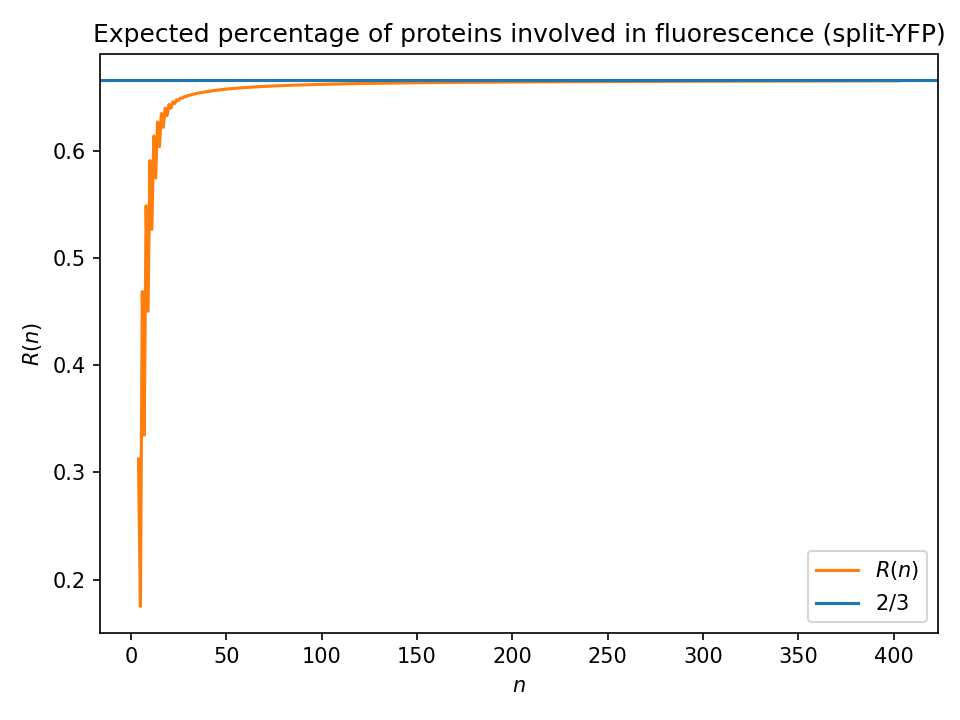
\includegraphics[width=0.75\textwidth]{SplitYFPamyloids.png}
\caption{$R_{\text{SY}}(n)$ for split-YFP amyloids. The blue line is $2/3$ and the orange curve is the exact $R_{\text{SY}}(n)$. Convergence to the limiting ratio is algebraic ($O(1/n)$), with a smaller alternating exponential correction.}
\label{fig:splityfp}
\end{figure}


\section{Introducing Sup35p into Amyloids}
We now want to consider the facts above but with the introduction of yeast prion protein Sup35p (which we label with an $S$) into our amyloids. In our model, Sup35p is treated as completely inert: it cannot participate in any fluorescent interaction, and its sole effect is to sterically separate adjacent split-YFP halves, preventing them from conjoining and fluorescing. Our amyloids can now be described using the regular expression $\{A,B,S\}^*$. We would like to first analyze the case where Sup35p and the halves of Split-YFP come in equal concentrations, and are thus equally likely to occur as the next protein in an amyloid sequence.

The 01 representation introduced in Section 2 must be extended to $\{A, B, S\}^n$ to reflect Sup35p's inertness. Applied verbatim, the Section 2 rule ``$f_i = 1$ iff $s_i \neq s_{i-1}$ and $f_{i-1} = 0$'' would mark an $S \to A$ adjacency as fluorescing, contradicting the modeling assumption that S blocks fluorescence. The intended rule, used implicitly throughout this section, is:
\[
f_i = \begin{cases}
0, & \text{if } i = 1, \\
1, & \text{if } i \ge 2,\ \{s_{i-1}, s_i\} = \{A, B\},\ \text{and}\ f_{i-1} = 0, \\
0, & \text{otherwise.}
\end{cases}
\]
That is, a 1 requires both proteins in the adjacency to be split-YFP halves (one A and one B), and that the left protein not already be consumed by a prior fusion. With this extension, the set of 01 patterns produced by $\{A,B,S\}^n$ sequences is exactly the same as in Section 2: the regular expression $(0^*01)^*0^*$ still describes all attainable patterns, since insertions of S only stretch existing zero runs.

\subsection{Number of distinct lighting patterns and 01 representations}
The introduction of Sup35p does not change this. When we abstract away the details we are still looking at 01 patterns of the form $(0^*01)^* 0^*$. Hence we have $F_{n+1}$ distinct lighting patterns for an amyloid of length $n$ (using the convention $F_1 = F_2 = 1$).

\subsection{Probability of $k$ fluorescing locations in length $n$ amyloid}\label{subsec:s3-dist}

We derive the joint distribution of length and fluorescence count from a bivariate generating function obtained by a two-state Markov decomposition, and then unpack it into a block-decomposition formula that mirrors Section 2.

\paragraph{Bivariate generating function.} Build an A-B-S amyloid one protein at a time, classifying its rightmost protein into two lumped states:
\begin{itemize}
\item \textbf{$p$}: rightmost is A or B and is not currently part of a fused pair.
\item \textbf{$q$}: rightmost is either S, or is A/B that has just been fused with its left neighbor.
\end{itemize}
The transitions, weighted by $z$ for length and $w$ for each fluorescing site produced, are:
\[
M(w) = \begin{pmatrix} 1 & 1 + w \\ 2 & 1 \end{pmatrix},
\]
where the rows index the from-state $(p, q)$ and the columns the to-state. From $p$ (say rightmost is A, unfused): next protein A yields one new amyloid ending in $p$ (weight $1$); next protein B fuses and yields one amyloid ending in $q$ (weight $w$, $+1$ fluorescence); next protein S yields one amyloid ending in $q$ (weight $1$). From $q$: either A or B sends us to $p$ (weight $2$ for two letters), and S sends us back to $q$ (weight $1$). By the A--B symmetry the two unfused sub-states merge consistently. Starting with the count vector $(2, 1)$ at $n = 1$ (two amyloids of length 1 in state $p$, namely A and B; one in state $q$, namely S), the joint generating function
\[
F(z, w) := \sum_{n \ge 0} \sum_{k \ge 0} \cA(n, k)\, w^k z^n
\]
(where in this section $\cA(n,k)$ counts amyloids over $\{A,B,S\}$, and $\cA(0, 0) := 1$ by convention) satisfies $F = 1 + z(2, 1) (I - z M(w))^{-1} (1, 1)^T$, which evaluates to
\begin{equation}\label{eq:s3-bivar-gf}
F(z, w) = \frac{1 + z}{1 - 2z - (1 + 2w)\,z^2}.
\end{equation}
Equivalently, the coefficients satisfy the recurrence $\cA(n, k) = 2\cA(n-1, k) + \cA(n-2, k) + 2\cA(n-2, k-1)$ with the appropriate small-$n$ initial conditions. Two specializations recover familiar facts. At $w = 0$, we count amyloids with no fluorescence: $F(z, 0) = (1+z)/(1 - 2z - z^2)$, whose coefficients $b_n$ enumerate A-B-S sequences with all-zero 01 representation. At $w = 1$, all amyloids are counted: $F(z, 1) = (1+z)/(1 - 2z - 3z^2) = 1/(1 - 3z)$ (after canceling the factor $1+z$ from $1 - 2z - 3z^2 = (1 - 3z)(1 + z)$), so $[z^n] F(z, 1) = 3^n$ as required.

The expected value $E(n)$ can now be extracted in a few lines from $\partial F / \partial w \big|_{w=1}$:
\[
\left.\frac{\partial F}{\partial w}\right|_{w = 1} = \frac{2 z^2 (1+z)}{(1 - 2z - 3z^2)^2} = \frac{2 z^2}{(1 - 3z)^2 (1 + z)},
\]
and partial-fraction expansion (carried out explicitly in Section~\ref{subsec:s3-Eq} below as a consistency check) yields the closed form
\[
E(n) \cdot 3^n = [z^n] \frac{2 z^2}{(1 - 3z)^2 (1 + z)} = \frac{3^{n-1}(4n - 3) + (-1)^n}{8}.
\]
Equivalently, $E(n) = (4n - 3)/24 + (-1)^n / (8 \cdot 3^n) = (4n-3)/24 - (-1)^{n-1}/(24 \cdot 3^{n-1})$, which is the same formula derived by the Markov chain argument in Section~\ref{subsec:s3-Eq}.

\paragraph{Block decomposition.} The bivariate generating function~(\ref{eq:s3-bivar-gf}) admits a more explicit reading via the regular-expression decomposition $(0^*01)^*0^*$ of the 01 pattern. Each amyloid of length $n$ with $k$ ones in its 01 pattern decomposes uniquely as $k$ consecutive ``active blocks'' of the form $0^+ 1$, followed by a trailing run of zeros:
\[
\underbrace{0\cdots 0\, 1}_{\phi_1} \; \underbrace{0\cdots 0\, 1}_{\phi_2} \; \cdots \; \underbrace{0\cdots 0\, 1}_{\phi_k} \; \underbrace{0\cdots 0}_{q}
\]
with $\phi_i \ge 2$ and $q \ge 0$. The protein choices within different blocks are independent: once block $i$ ends with a fusion at position $j$ (so $s_j$ is consumed by the previous fusion), the protein at position $j+1$ may be any of $\{A, B, S\}$ unconstrained, since $f_{j+1} = 0$ is forced regardless of $s_{j+1}$. Hence the number of amyloids realizing a given block decomposition factors:
\begin{equation}\label{eq:s3-blockcount}
\cA(n,k) = \sum_{q=0}^{n - 2k} b_q \sum_{\substack{\phi_1 + \cdots + \phi_k = n-q \\ \phi_i \ge 2}} \prod_{i=1}^k a_{\phi_i},
\end{equation}
where $a_\phi$ counts A-B-S patterns of length $\phi$ whose 01 representation is $0^{\phi-1} 1$, and $b_q$ counts patterns of length $q$ with all-zero 01 representation. For $k=0$, the formula reduces to the all-zero case $\cA(n,0)=b_n$. Thus $P(n,k)=\cA(n,k)/3^n$. Equation~(\ref{eq:s3-blockcount}) is the convolutional unfolding of~(\ref{eq:s3-bivar-gf}): writing $F(z, w) = B(z) / (1 - w\, A(z))$ with $A(z) = \sum_{\phi \ge 2} a_\phi z^\phi = 2 z^2 / (1 - 2z - z^2)$ and $B(z) = \sum_{q \ge 0} b_q z^q = (1+z)/(1 - 2z - z^2)$, one verifies
\[
\frac{B(z)}{1 - w A(z)} = \frac{(1+z)/(1 - 2z - z^2)}{1 - 2 w z^2/(1 - 2z - z^2)} = \frac{1 + z}{1 - 2z - (1 + 2w) z^2},
\]
recovering (\ref{eq:s3-bivar-gf}).

\paragraph{The sequences $a_n$ and $b_n$.} Both sequences are governed by the same denominator $1 - 2x - x^2$. From the regular expressions $S^* \{AA^* SS^*, BB^* SS^*\}^* \{AA^*, BB^*, \varepsilon\}$ for the $b$-sequence and $S^* \{AA^* SS^*, BB^* SS^*\}^* \{AA^*B, BB^*A\}$ for the $a$-sequence (setting $A = B = S = x$ throughout), one obtains the ordinary generating functions
\[
\sum_{n \ge 0} b_n x^n = \frac{1 + x}{1 - 2x - x^2}, \qquad \sum_{n \ge 0} a_n x^n = \frac{2 x^2}{1 - 2x - x^2},
\]
yielding the recurrences $b_n = 2 b_{n-1} + b_{n-2}$ for $n \ge 2$ (with $b_0 = 1$, $b_1 = 3$) and $a_n = 2 a_{n-1} + a_{n-2}$ for $n \ge 3$ (with $a_0 = a_1 = 0$, $a_2 = 2$). The denominator's roots are reciprocals of $1 \pm \sqrt{2}$, and clean partial-fraction decomposition gives the closed forms
\begin{align}
b_n &= \frac{(1 + \sqrt{2})^{n+1} + (1 - \sqrt{2})^{n+1}}{2}, \quad n \ge 0, \label{eq:s3-bn-closed} \\[4pt]
a_n &= \left(1 + \tfrac{\sqrt{2}}{2}\right)(1 - \sqrt{2})^n + \left(1 - \tfrac{\sqrt{2}}{2}\right)(1 + \sqrt{2})^n, \quad n \ge 1 \label{eq:s3-an-closed}
\end{align}
(the formula for $a_n$ does not extend to $n = 0$, where it gives $2$ rather than $a_0=0$; this is absorbed by the non-homogeneous initial conditions). Both sequences appear in OEIS: $b_n = $ A001333$(n+1)$ and $a_n / 2 = $ A000129$(n-1)$ for $n \ge 1$, where A001333 and A000129 are respectively the continued-fraction numerators of $\sqrt{2}$ and the Pell numbers. Verification: $a_2 = (1 + \sqrt{2}/2)(3 - 2\sqrt{2}) + (1 - \sqrt{2}/2)(3 + 2\sqrt{2}) = 6 - (\sqrt{2}/2)(4\sqrt{2}) = 6 - 4 = 2$; $b_0 = (1+\sqrt{2} + 1-\sqrt{2})/2 = 1$. The first values are $b_0, b_1, \ldots = 1, 3, 7, 17, 41, 99, \ldots$ and $a_0, a_1, \ldots = 0, 0, 2, 4, 10, 24, \ldots$

\textbf{Worked example.} For $n = 4$, $k = 1$, the block decomposition has one block of length $\phi_1 \ge 2$ followed by a tail of length $q = 4 - \phi_1$:
\begin{center}
\begin{tabular}{cccc}
$\phi_1$ & $q$ & 01 pattern & $a_{\phi_1} \cdot b_q$ \\
\hline
2 & 2 & 0100 & $2 \cdot 7 = 14$ \\
3 & 1 & 0010 & $4 \cdot 3 = 12$ \\
4 & 0 & 0001 & $10 \cdot 1 = 10$ \\
\end{tabular}
\end{center}
So $\cA(4,1) = 14 + 12 + 10 = 36$, confirmed by brute-force enumeration. Cross-checking against~(\ref{eq:s3-bivar-gf}): the coefficient of $z^4 w^1$ in $F(z, w)$, computed via the recurrence, equals $36$ as well.


\subsection{Expected number of fluorescing locations}

This is simply the sum:

\[
    E(n) = \frac{1}{3^n}\sum_{k=1}^{\floor{n/2}} k \cdot \cA(n,k)
\]

by definition of expected value.

\subsection{Expected percentage of proteins involved in fluorescence}\label{subsec:s3-Eq}

This is the number:

\[
    R_{\text{SY}}(n) = \frac{2E(n)}{n}
\]

We prove that $\lim_{n \to \infty} R_{\text{SY}}(n) = 1/3$ by computing $E(n)$ directly using a Markov chain argument, bypassing the combinatorial formula for $\cA(n,k)$.

Consider building an amyloid one protein at a time, where each protein is independently A, B, or S with equal probability $1/3$. We define two states based on the status of the most recently added protein:
\begin{itemize}
\item \textbf{State $p$}: the rightmost protein is A or B and is \textit{not} part of a fused pair (and so is available to fuse with the next protein).
\item \textbf{State $q$}: the rightmost protein is either S, or is A/B but already part of a fused pair (and so the next protein cannot fuse with it).
\end{itemize}

The transition probabilities are as follows. From state $p$ (say the rightmost protein is A, unfused):
\begin{itemize}
\item With probability $1/3$, the next protein is A (same type): no fusion, go to $p$.
\item With probability $1/3$, the next protein is B (different type): fusion occurs (+1 fluorescence), go to $q$.
\item With probability $1/3$, the next protein is S: no fusion, go to $q$.
\end{itemize}
By symmetry between A and B, the case where the rightmost is B is identical. So from $p$: transition to $p$ with probability $1/3$, to $q$ with probability $2/3$, with expected fluorescence $1/3$.

From state $q$, the rightmost protein cannot fuse regardless of the next protein's type. The next protein is A, B, or S each with probability $1/3$, and is always unfused. So from $q$: transition to $p$ with probability $2/3$ (next is A or B), to $q$ with probability $1/3$ (next is S), with expected fluorescence $0$.

Let $p_n$ denote the probability of being in state $p$ after the $n$th protein. The initial state is $p$ with probability $2/3$ and $q$ with probability $1/3$, so $p_1 = 2/3$. The recurrence is:
\[
p_{n+1} = \frac{1}{3} p_n + \frac{2}{3}(1 - p_n) = \frac{2}{3} - \frac{1}{3} p_n
\]
This has fixed point $p^* = 1/2$, and the general solution is
\[
p_n = \frac{1}{2} + \frac{(-1/3)^{n-1}}{6}
\]
which is verified by checking $p_1 = 1/2 + 1/6 = 2/3$.

The expected fluorescence contributed by the $(n+1)$th protein is $e_{n+1} = p_n / 3$, so
\begin{align*}
E(n) &= \sum_{i=2}^{n} e_i = \frac{1}{3} \sum_{j=1}^{n-1} p_j = \frac{1}{3} \sum_{j=1}^{n-1} \left[ \frac{1}{2} + \frac{(-1/3)^{j-1}}{6} \right] \\
&= \frac{n-1}{6} + \frac{1}{18} \cdot \frac{1 - (-1/3)^{n-1}}{4/3} = \frac{n-1}{6} + \frac{1}{24}\left(1 - (-1/3)^{n-1}\right) \\
&= \frac{4n - 3}{24} - \frac{(-1)^{n-1}}{24 \cdot 3^{n-1}}
\end{align*}

Therefore
\[
R_{\text{SY}}(n) = \frac{2E(n)}{n} = \frac{4n-3}{12n} + \frac{(-1)^n}{12n \cdot 3^{n-1}}
\]

and as $n \to \infty$, the second term vanishes:
\[
\lim_{n \to \infty} R_{\text{SY}}(n) = \lim_{n \to \infty} \frac{4n - 3}{12n} = \frac{4}{12} = \frac{1}{3}
\]

As in Section 2, the agreement between the Markov chain and the combinatorial formula provides a non-trivial identity. Since both methods compute $E(n)$, we have
\[
\frac{1}{3^n} \sum_{k=1}^{\floor{n/2}} k \cdot \cA(n,k) = \frac{4n-3}{24} - \frac{(-1)^{n-1}}{24 \cdot 3^{n-1}}
\]
where $\cA(n,k)$ is the combinatorial formula involving the $a_{\phi_i}$ and $b_q$ sequences with $\sqrt{2}$. The left-hand side is the definition of $E(n)$, and the right-hand side is the Markov chain result derived in closed form above. Since both are proven independently---the combinatorial formula for $\cA(n,k)$ via generating functions on regular expressions, and $E(n)$ via the Markov recurrence---their equality is established, not merely conjectured. This identity, which equates a sum over compositions weighted by products of irrational-valued sequences to a simple rational expression, can also be numerically verified: at $n = 4$, the left-hand side gives $(1 \cdot 36 + 2 \cdot 4)/81 = 44/81$, and the right-hand side gives $(4 \cdot 4 - 3)/24 + 1/(24 \cdot 27) = 13/24 + 1/648 = 44/81$. $\checkmark$

A simulation (see \texttt{sup35\_simulation.py}) confirms this. A sample of computed values is shown in Table~\ref{tab:sup35}, and the graph appears in Figure~\ref{fig:sup35}.

\begin{table}[ht]
\centering
\begin{tabular}{rc|rc|rc}
\hline
$n$ & $R_{\text{SY}}(n)$ & $n$ & $R_{\text{SY}}(n)$ & $n$ & $R_{\text{SY}}(n)$ \\
\hline
2 & 0.222222 & 10 & 0.308334 & 20 & 0.320833 \\
3 & 0.246914 & 11 & 0.310606 & 25 & 0.323333 \\
4 & 0.271605 & 12 & 0.312500 & 50 & 0.328333 \\
5 & 0.283128 & 13 & 0.314103 & 100 & 0.330833 \\
6 & 0.291724 & 14 & 0.315476 & 200 & 0.332083 \\
7 & 0.297603 & 15 & 0.316667 & 400 & 0.332708 \\
\hline
\multicolumn{6}{c}{$R_{\text{SY}}(n) \to 1/3 \approx 0.333333$} \\
\end{tabular}
\caption{Sample values of $R_{\text{SY}}(n)$ for split-YFP amyloids with Sup35p.}
\label{tab:sup35}
\end{table}

\begin{figure}[ht]
\centering

\includegraphics[width=0.75\textwidth]{splityfpandsup35.png}
\caption{$R_{\text{SY}}(n)$ for split-YFP amyloids with Sup35p. The blue line is $1/3$ and the orange curve is the exact $R_{\text{SY}}(n)$. Convergence to the limiting ratio is algebraic ($O(1/n)$), with a smaller alternating exponential correction.}
\label{fig:sup35}
\end{figure}


\section{Using FRET in amyloids of YFP and CFP}\label{sec:fret}

Consider the case where full YFP (i.e., both halves are conjoined to form the complete fluorophore) and CFP are well-mixed in a container under ambient lighting that causes CFP to fluoresce. When CFP is bonded to YFP, the fluorescence from CFP will cause YFP to fluoresce (FRET). 

We are interested in measuring the \textit{total} yellow fluorescence emanating from amyloids of this kind. That is, the YFPs may fluoresce at a fixed level (call it Level 1) when it is next to one and only one CFP, but it may also fluoresce twice as much (Level 2) if it is next to \textit{two} CFPs as in a YFP being sandwiched between two CFPs. We want to then sum over the total yellow fluorescence of an amyloid rather than just the raw number of YFPs that are caused to fluoresce. We note that this additive model of FRET from multiple donors is a mathematical idealization; in practice, the efficiency of energy transfer from two donors to a single acceptor depends on geometric factors beyond simple adjacency. We adopt this convention for analytical tractability. A more realistic model incorporating geometry-dependent FRET efficiencies would require replacing the simple adjacent-pair counting argument below with a specified physical contribution model.

Label YFP as Y and CFP as C. The blocking constraint $f_{i-1} = 0$ that was central to Sections 2 and 3 does \emph{not} apply here: a YFP can fluoresce simultaneously from both of its CFP neighbors (additively, by our convention), so consecutive 1s in the 01 representation are allowed. The Section 4--5 definition of the 01 pattern is accordingly
\[
f_i = \begin{cases}
0, & \text{if } i = 1, \\
1, & \text{if } i \ge 2 \text{ and } \{s_{i-1}, s_i\} = \{C, Y\}, \\
0, & \text{otherwise,}
\end{cases}
\]
with no constraint on $f_{i-1}$. Then our patterns are $\{Y,C\}^*$ and, extracting away the details, we get patterns of the form $(0^* 0 1^*1)^* 0^*$, which generates all binary strings of length $n$ beginning with $0$---that is, all $2^{n-1}$ such strings. Here we write a $1$ whenever the full protein at that location causes the previous to fluoresce OR is caused to fluoresce by the previous. We note that, unlike previous cases, once we fix the first protein (Y or C), the 01 pattern uniquely determines every subsequent protein: a $1$ forces the next protein to differ from its predecessor, while a $0$ forces it to match. Therefore, for each 01 pattern there are exactly 2 Y-C sequences (one starting with Y, one with C).

It is now remarked that there is a one-to-one correspondence between 1's as appearing in 0-1 patterns as described above and the total yellow fluorescence emanating from an amyloid of the kind. To be specific, the number of 1's is equal to the total yellow fluorescence (if we take Level 1 to be 1 and Level 2 to be 2 as numerical values for which we sum up). For example:

\begin{alignat}{11}
\text{$\{C, Y \}^*$:  } & C & Y & Y & Y & C & Y & C & Y & Y & C  & C \\
\text{$(0^*0 1^* 1)^* 0^*$:  } & 0 & 1 & 0 & 0 & 1 & 1 & 1 & 1 & 0 & 1 & 0 \\
\text{Yellow fluorescence:  } & 0 & 1 & 0 & 1 & 0 & 2 & 0 & 1 & 1 & 0 & 0
\end{alignat}
Note that in the 01 pattern, each $1$ is attributed to the right endpoint of a $\{C,Y\}$ adjacency as a bookkeeping convention, not to the physically emitting protein. The key claim is that the \textit{total} number of $1$s equals the total yellow fluorescence, which we verify: both rows sum to $6$.

\subsection{Probability of $k$ total yellow fluorescence in length $n$ amyloid}

The number of amyloids of length $n$ with $k$ total yellow fluorescence is:

\[
\cA(n,k) = 2\binom{n-1}{k}, \quad k \in [0,n - 1]
\]

and thus the probability of observing $k$ total yellow fluorescence in a length $n$ amyloid is


\[
P(n,k) = \frac{2\binom{n-1}{k}}{2^n} = \frac{\binom{n-1}{k}}{2^{n-1}}, \quad k \in [0,n - 1]
\].

This is the Binomial$(n-1, 1/2)$ distribution, which can also be seen directly. Let $\varepsilon_i = \pm 1$ according to whether protein $i$ is C or Y, and define $d_i = \varepsilon_i \cdot \varepsilon_{i-1}$ for $i \ge 2$. Then $f_i = 1$ iff $d_i = -1$. The map $(\varepsilon_1, \ldots, \varepsilon_n) \mapsto (\varepsilon_1, d_2, \ldots, d_n)$ is a bijection on $\{\pm 1\}^n$ (since $\varepsilon_i = \varepsilon_1 \prod_{j=2}^i d_j$ is recoverable), so $(d_2, \ldots, d_n)$ are mutually independent and uniform on $\{\pm 1\}$. Hence $f_2, \ldots, f_n$ are mutually independent Bernoulli$(1/2)$ despite their overlapping definition, and their sum is Binomial$(n-1, 1/2)$.

\subsection{Expected total yellow fluorescence}

This is simply the sum:

\[
    E(n) = \sum_{k = 0}^{n - 1} k \cdot P(n,k) 
\]

by definition of expected value.

Note that, by a standard identity \cite[\S 5.1, Eq.~5.5]{gkp1994}:

\begin{align*}
E(n) := \frac{1}{2^{n-1}} \cdot \sum_{k=0}^{n - 1} k \cdot \binom{n-1}{k} 
 =  \frac{1}{2^{n-1}} \cdot (n-1) 2^{n-2} = \frac{n - 1}{2}
\end{align*}

So that for very large $n$, we expect to see about as much yellow unit fluorescence as half the length of the amyloid.

Note that $E(n) = (n-1)/2$ also follows directly from linearity of expectation: the total yellow fluorescence equals the number of adjacent $\{C,Y\}$ pairs, and there are $n - 1$ adjacent pairs each with probability $P(\{C,Y\}) = 2 \cdot (1/2)^2 = 1/2$ of being a $\{C,Y\}$ pair (since FRET interactions, unlike split-YFP fusion, have no blocking constraint). We define the fluorescence ratio as
\[
R_{\text{F}}(n) := E(n)/n = \frac{n-1}{2n} \longrightarrow \frac{1}{2} \text{ as } n \to \infty
\]

The first 400 values of $R_{\text{F}}(n)$ appear in Figure~\ref{fig:fretonly}.

\begin{figure}[ht]
\centering
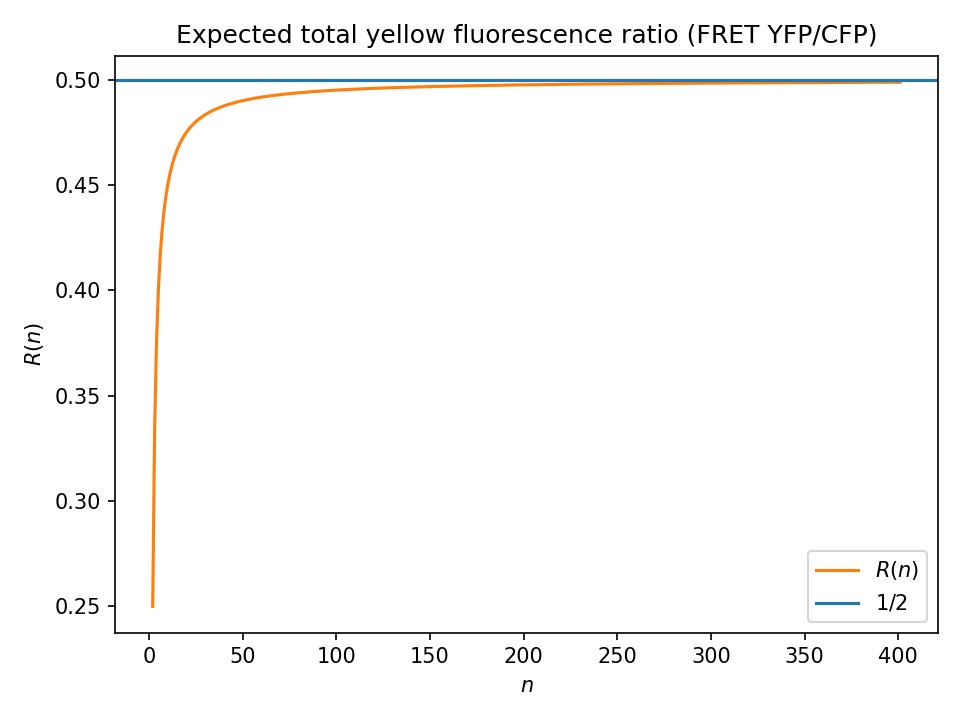
\includegraphics[width=0.75\textwidth]{FretOnly.png}
\caption{$R_{\text{F}}(n)$ for FRET YFP/CFP amyloids. The blue line is $1/2$ and the orange curve is the exact $R_{\text{F}}(n) = (n-1)/(2n)$. Convergence is algebraic ($O(1/n)$), with no exponential correction.}
\label{fig:fretonly}
\end{figure}

\section{Using FRET in amyloids of YFP, CFP, and Sup35p}\label{sec:fret-sup35}
As with section 3, we will now analyze the case of introducing Sup35p to the system in Section 4. That is, we have Sup35p, YFP, and CFP well mixed and of equal concentrations in a container under ambient lighting which causes CFP to fluoresce. The cyan fluorescence of a CFP will cause an adjacent YFP to fluoresce yellow due to FRET, and this fluorescence can be stacked so that a YFP sandwiched between two CFPs will fluoresce twice as much as in the case where a YFP is next to only 1 CFP. The presence of Sup35p will block the YFPs and CFPs from interacting under FRET.

Our pattern becomes $\{C,Y,S \}^*$ where $C$ represents CFP, $Y$ represents YFP, and $S$ represents Sup35p. The 01 pattern is still $(0^* 0 1^*1)^* 0^*$ as before. 

\subsection{Probability of $k$ total yellow fluorescence in length $n$ amyloid}

The block-decomposition approach used for Section~\ref{subsec:s3-dist} does not transfer cleanly to this setting. The reason is that, unlike split-YFP fusion, FRET allows consecutive 1s in the 01 pattern (a YFP sandwiched between two CFPs fluoresces twice), so each block has the form $0^+ 1^+$ rather than $0^+ 1$. The last protein of a $1^+$ run is always in $\{C, Y\}$, and the first protein of the next block must form $f = 0$ with it---hence must match it or be S, only 2 choices among $\{C, Y, S\}$. This boundary coupling means a block decomposition would need to carry boundary-state information; the transfer matrix is the simpler way to track the rightmost protein type.

\paragraph{Bivariate generating function.} Lump $\{C, Y\}$ into a single state (justified by the $C \leftrightarrow Y$ symmetry of the model under equal concentrations), and track two states by the rightmost protein type:
\begin{itemize}
\item \textbf{$p$}: rightmost is C or Y.
\item \textbf{$q$}: rightmost is S.
\end{itemize}
The weighted transition matrix (rows = from, cols = to; $z$ marks length, $w$ marks each fluorescing site) is
\[
M(w) = \begin{pmatrix} 1 + w & 1 \\ 2 & 1 \end{pmatrix}.
\]
From $p$ (say rightmost is C): next protein C stays in $p$ with no fluorescence (weight $1$); next protein Y stays in $p$ but produces a fluorescence (weight $w$); next protein S goes to $q$ (weight $1$). By $C \leftrightarrow Y$ symmetry the rightmost-Y case is symmetric. From $q$ (rightmost is S): C and Y carry no fluorescence with S, so next $\in \{C, Y\}$ takes us to $p$ (combined weight $2$), and next $= S$ stays in $q$ (weight $1$). Starting from the count vector $(2, 1)$ at $n = 1$, the joint generating function
\[
F_{\text{F},S}(z, w) := \sum_{n \ge 0} \sum_{k \ge 0} \cA(n, k)\, w^k z^n
\]
(with $\cA(0, 0) := 1$) is
\begin{equation}\label{eq:s5-bivar-gf}
F_{\text{F},S}(z, w) = \frac{1 + (1 - w)\, z}{1 - (2 + w)\, z - (1 - w)\, z^2}.
\end{equation}
Equivalently, the coefficients satisfy the recurrence $f_n = (2 + w)\, f_{n-1} + (1 - w)\, f_{n-2}$ with $f_0 = 1$, $f_1 = 3$. At $w = 0$ this recovers $F_{\text{F},S}(z, 0) = (1 + z)/(1 - 2z - z^2)$, the same denominator as $b_n$ in Section~\ref{subsec:s3-dist}---which is correct, since both sequences count length-$n$ A-B-S (or C-Y-S) strings with no fluorescent adjacency, regardless of alphabet relabeling. At $w = 1$ the generating function becomes $F_{\text{F},S}(z,1)=1/(1-3z)$, so $[z^n]F_{\text{F},S}(z,1)=3^n$ as required.

The denominator factors as $(1 - \lambda_+ z)(1 - \lambda_- z)$ where the eigenvalues of $M(w)$ are
\[
\lambda_\pm(w) = 1 + \frac{w \pm \sqrt{w^2 + 8}}{2},
\]
recovering $\lambda_+(1) = 3$, $\lambda_-(1) = 0$, and $\lambda_\pm(0) = 1 \pm \sqrt{2}$ consistently with the $w = 0, 1$ specializations.

\paragraph{Expected value via $\partial F_{\text{F},S}/\partial w$.} Differentiating~(\ref{eq:s5-bivar-gf}) in $w$ and evaluating at $w = 1$ gives, after simplification,
\[
\left.\frac{\partial F_{\text{F},S}}{\partial w}\right|_{w = 1} = \frac{2 z^2}{(1 - 3z)^2}.
\]
Hence
\[
E(n) \cdot 3^n = [z^n] \frac{2 z^2}{(1 - 3z)^2} = 2 (n - 1)\, 3^{n - 2}, \qquad n \ge 2,
\]
giving $E(n) = 2(n-1)/9$ exactly, with no exponential correction term. This matches the linearity-of-expectation derivation given below.

\textbf{Verification.} For $n = 3$, brute-force enumeration over all $3^3 = 27$ amyloids in $\{C,Y,S\}^3$ gives $\cA(3,0) = 17$, $\cA(3,1) = 8$, and $\cA(3,2) = 2$, with $E(3) = (0 \cdot 17 + 1 \cdot 8 + 2 \cdot 2)/27 = 12/27 = 4/9$. This agrees with both the linearity-of-expectation formula $E(3) = 2(3-1)/9 = 4/9$ and the generating-function expansion: $[z^3] F_{\text{F},S}(z, w) = 17 + 8w + 2w^2$ by direct computation of the recurrence $f_n = (2+w) f_{n-1} + (1-w) f_{n-2}$. For $n = 4$, both routes give $\cA(4, k) = 41, 28, 10, 2$ for $k = 0, 1, 2, 3$, with $E(4) = (28 + 20 + 6)/81 = 54/81 = 2/3 = 2 \cdot 3 / 9$ as expected. (See \texttt{verify\_section5\_gf.py}.)

The bivariate generating function above encodes the full probability distribution via $P(n,k)=\cA(n,k)/3^n$. However, for computing the expected value, a much simpler route is available. As in Section 4, the total yellow fluorescence of an amyloid equals the number of adjacent $\{C,Y\}$ pairs. Since FRET interactions have no blocking constraint (unlike split-YFP fusion), the linearity of expectation argument from Section 4 applies directly. With each protein independently C, Y, or S with probability $1/3$:
\[
E(n) = (n-1) \cdot P(\{C,Y\} \text{ pair}) = (n-1) \cdot 2 \cdot \frac{1}{3} \cdot \frac{1}{3} = \frac{2(n-1)}{9}
\]

Therefore
\[
R_{\text{F}}(n) := E(n)/n = \frac{2(n-1)}{9n} \longrightarrow \frac{2}{9} \text{ as } n \to \infty
\]

The first 400 values of $R_{\text{F}}(n)$ appear in Figure~\ref{fig:fretsup35}.

\begin{figure}[ht]
\centering
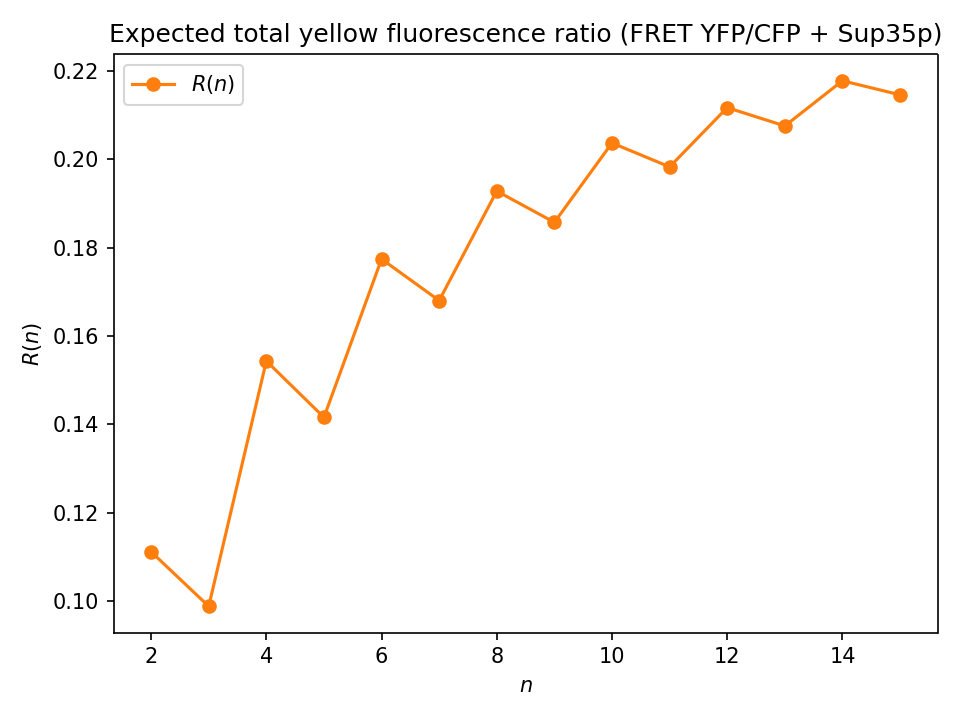
\includegraphics[width=0.75\textwidth]{FretandSup35.png}
\caption{$R_{\text{F}}(n)$ for FRET YFP/CFP amyloids with Sup35p. The blue line is $2/9$ and the orange curve is the exact $R_{\text{F}}(n) = 2(n-1)/(9n)$. Convergence is algebraic ($O(1/n)$), as in Figure~\ref{fig:fretonly}.}
\label{fig:fretsup35}
\end{figure}

\section{Variance, error bars, and finite-radius FRET}\label{sec:variance-radius}

The preceding sections emphasize exact expectations, but the same probability distributions also give exact finite-$n$ fluctuations. Let $K_n$ denote the fluorescence count in the relevant model. If
\[
F(z,w) = \sum_{n \ge 0} \sum_{k \ge 0} \cA(n,k) w^k z^n
\]
is the corresponding bivariate generating function and $T_n$ is the total number of amyloids of length $n$, then
\[
E[K_n] = \frac{[z^n]F_w(z,1)}{T_n}, \qquad
E[K_n(K_n-1)] = \frac{[z^n]F_{ww}(z,1)}{T_n},
\]
and hence
\[
\operatorname{Var}(K_n) = E[K_n(K_n-1)] + E[K_n] - E[K_n]^2.
\]
For the exclusively split-YFP model, the bivariate generating function is
\[
F_{\text{SY}}(z,w) = \frac{1+z}{1-z-2wz^2},
\]
obtained from the same two-state decomposition as in Section~2. In transfer-matrix form, with $p$ denoting an unfused A/B endpoint and $q$ denoting a fused endpoint, the weighted transition matrix is
\[
M_{\text{SY}}(w)=
\begin{pmatrix}
1 & w\\
2 & 0
\end{pmatrix},
\]
where the rows and columns are ordered as $(p,q)$ and $w$ marks a fusion. Including the empty amyloid and the initial vector $(2,0)$ gives
\[
F_{\text{SY}}(z,w)=1+z(2,0)\left(I-zM_{\text{SY}}(w)\right)^{-1}\binom{1}{1}
=\frac{1+z}{1-z-2wz^2}.
\]
Its second derivative at $w=1$ is
\[
\left. \frac{\partial^2 F_{\text{SY}}}{\partial w^2} \right|_{w=1}
= \frac{8z^4}{(1-2z)^3(1+z)^2}.
\]
Using this together with the expectation from Section~2 gives, for $n \ge 2$,
\[
\operatorname{Var}_{\text{SY}}(K_n)
=
\frac{6n+2}{81}
+
\frac{(12n+2)(-1)^n}{81\cdot 2^n}
-
\frac{4}{81\cdot 4^n}.
\]
For split-YFP with Sup35p, differentiating~(\ref{eq:s3-bivar-gf}) twice gives
\[
\left. \frac{\partial^2 F}{\partial w^2} \right|_{w=1}
= \frac{8z^4}{(1-3z)^3(1+z)^2},
\]
and therefore
\[
\operatorname{Var}_{\text{SY},S}(K_n)
=
\frac{56n-27}{576}
+
\frac{(4n+3)(-1)^n}{48\cdot 3^n}
-
\frac{1}{64\cdot 9^n},
\qquad n \ge 2.
\]
For FRET without Sup35p, Section~4 identifies $K_n$ as a Binomial$(n-1,1/2)$ random variable, so
\[
\operatorname{Var}_{\text{F}}(K_n)=\frac{n-1}{4}.
\]
For FRET with Sup35p, differentiating~(\ref{eq:s5-bivar-gf}) twice gives
\[
\left. \frac{\partial^2 F_{\text{F},S}}{\partial w^2} \right|_{w=1}
= \frac{4z^3(1-z)}{(1-3z)^3},
\]
which yields
\[
\operatorname{Var}_{\text{F},S}(K_n)=\frac{18n-22}{81},
\qquad n \ge 2.
\]
As a small check, at $n=2$ the split-YFP and FRET-with-Sup35p distributions are both $(7,2)/9$ on $K_2=0,1$, giving variance $14/81$, exactly as the formulas above do. The accompanying script \texttt{verify\_variance.py} also brute-force checks these variance formulas for small $n$.

These formulas turn the expected fluorescence ratios into exact null-model error bars. Since $R_{\text{SY}}(n)=2K_n/n$ in the split-YFP models and $R_{\text{F}}(n)=K_n/n$ in the FRET models,
\[
\operatorname{Var}(R_{\text{SY}}(n)) = \frac{4}{n^2}\operatorname{Var}(K_n), \qquad
\operatorname{Var}(R_{\text{F}}(n)) = \frac{1}{n^2}\operatorname{Var}(K_n).
\]
Thus, for large $n$, the standard deviations of the ratio statistics scale as $O(n^{-1/2})$. For example,
\[
\operatorname{Var}(R_{\text{SY}}(n)) \sim \frac{8}{27n}, \quad
\operatorname{Var}(R_{\text{SY},S}(n)) \sim \frac{7}{18n}, \quad
\operatorname{Var}(R_{\text{F}}(n)) \sim \frac{1}{4n}, \quad
\operatorname{Var}(R_{\text{F},S}(n)) \sim \frac{2}{9n}.
\]
These finite-$n$ variances characterize the scale of random fluctuations under the i.i.d.\ null model. For short amyloids, the exact distributions $P(n,k)$ should be used directly; for experimental ensembles of many fibrils, the relevant uncertainty also depends on the sampling design and the number of fibrils measured.

The nearest-neighbor FRET assumption can also be relaxed at the level of expected value. Suppose a YFP can receive FRET from CFPs within distance $r$ along the amyloid, with additive unit contribution from each CFP--YFP pair in this window. Let $p_C$ and $p_Y$ be the probabilities of CFP and YFP, and set $m=\min(r,n-1)$. There are $n-d$ unordered pairs at distance $d$, each contributing in expectation $2p_Cp_Y$. Hence
\[
E_r(n) = 2p_Cp_Y \sum_{d=1}^{m} (n-d)
= 2p_Cp_Y\left(mn-\frac{m(m+1)}{2}\right).
\]
For fixed $r$ and $n \to \infty$, this gives
\[
\frac{E_r(n)}{n} \longrightarrow 2r p_Cp_Y.
\]
In the equal-concentration FRET+Sup35p case ($p_C=p_Y=1/3$), the nearest-neighbor model $r=1$ recovers $E_1(n)=2(n-1)/9$, while $r=2$ gives
\[
E_2(n)=\frac{2}{9}\bigl((n-1)+(n-2)\bigr)=\frac{4n-6}{9}, \qquad n \ge 3,
\]
and $E_2(n)/n \to 4/9$. Computing the full distribution for $r>1$ is substantially harder: adjacent indicators are correlated over a larger window, and a transfer matrix would need to track the last $r$ protein identities rather than only the rightmost state.

\section{Generalization to unequal concentrations}\label{sec:unequal}

The results of Sections 2--5 all depend on the equal-concentration assumption. The Markov chain arguments generalize readily to unequal concentrations, which we outline here.

\subsection{Split-YFP with unequal concentrations}
Suppose protein A appears with probability $\alpha$ and protein B with probability $1 - \alpha$. A two-state chain on $\{$unfused$, $ fused$\}$ is insufficient here, because the probability that the next protein triggers a fusion conditional on the current rightmost being unfused depends on whether the rightmost is an A or a B: from rightmost-A, fusion requires next = B (probability $1 - \alpha$), while from rightmost-B it requires next = A (probability $\alpha$). For $\alpha \neq 1/2$ these are not equal, so we cannot lump A-unfused and B-unfused into a single state without loss. We instead use the three-state chain $\{p_A, p_B, q\}$ from Section~\ref{subsec:unequal-sup35}, specialized to the no-Sup35p case $\beta = 1 - \alpha$ (so $1 - \alpha - \beta = 0$). The transitions are:
\begin{itemize}
\item From $p_A$: next is A (prob $\alpha$, stay $p_A$); next is B (prob $1{-}\alpha$, fuse, go $q$).
\item From $p_B$: next is B (prob $1{-}\alpha$, stay $p_B$); next is A (prob $\alpha$, fuse, go $q$).
\item From $q$: next is A (prob $\alpha$, go $p_A$); next is B (prob $1{-}\alpha$, go $p_B$).
\end{itemize}
The balance equations $\pi_A = \alpha \pi_A + \alpha \pi_q$ and $\pi_B = (1{-}\alpha)\pi_B + (1{-}\alpha)\pi_q$, together with $\pi_A + \pi_B + \pi_q = 1$, give
\[
\pi_A = \frac{\alpha^2}{1 - \alpha(1-\alpha)}, \qquad \pi_B = \frac{(1-\alpha)^2}{1 - \alpha(1-\alpha)}, \qquad \pi_q = \frac{\alpha(1-\alpha)}{1 - \alpha(1-\alpha)}.
\]
The expected fluorescence per step is $e = (1-\alpha)\pi_A + \alpha\pi_B = \alpha(1-\alpha)/(1 - \alpha(1-\alpha))$, so
\[
\lim_{n \to \infty} R_{\text{SY}}(n) = 2e = \frac{2\alpha(1-\alpha)}{1 - \alpha(1-\alpha)}.
\]
Equivalently, this is the specialization $\beta = 1 - \alpha$ of the Section~\ref{subsec:unequal-sup35} formula $2\alpha\beta(2-\alpha-\beta)/(1-\alpha\beta)$. At $\alpha = 1/2$, $R_{\text{SY}} \to (1/2)/(3/4) = 2/3$, recovering Section 2. The maximum occurs at equal concentrations: differentiating gives
\[
\frac{d}{d\alpha}\left(\frac{2\alpha(1-\alpha)}{1-\alpha(1-\alpha)}\right)
= \frac{2(1-2\alpha)}{(1-\alpha(1-\alpha))^2},
\]
so the only interior critical point is $\alpha=1/2$, and the endpoints have zero fluorescence. Numerically, at $\alpha = 1/4$ the limit is $2 \cdot \tfrac{3}{16} / \tfrac{13}{16} = 6/13 \approx 0.462$, in agreement with Monte Carlo simulation (see \texttt{split\_yfp\_unequal\_simulation.py}). A naive two-state chain would wrongly lump $p_A$ and $p_B$ into a single unfused state and assign fusion probability $d=2\alpha(1-\alpha)$ from that lumped state, giving the ratio $2d/(1+d)=4\alpha(1-\alpha)/(1+2\alpha(1-\alpha))$; at $\alpha = 1/4$ this is $6/11 \approx 0.545$. The two-state lumping is harmless at $\alpha=1/2$, where the A and B sub-states are symmetric, but it fails the simulation check at every $\alpha \neq 1/2$.

\subsection{Split-YFP with Sup35p at unequal concentrations}\label{subsec:unequal-sup35}
Now suppose proteins A, B, S appear with probabilities $\alpha$, $\beta$, and $1 - \alpha - \beta$ respectively. We define three Markov states: $p_A$ (rightmost is A, unfused), $p_B$ (rightmost is B, unfused), and $q$ (rightmost is S, or fused). The transitions are:
\begin{itemize}
\item From $p_A$: next is A (prob $\alpha$, stay $p_A$), B (prob $\beta$, fuse, go $q$), or S (prob $1{-}\alpha{-}\beta$, go $q$).
\item From $p_B$: next is B (prob $\beta$, stay $p_B$), A (prob $\alpha$, fuse, go $q$), or S (prob $1{-}\alpha{-}\beta$, go $q$).
\item From $q$: next is A (prob $\alpha$, go $p_A$), B (prob $\beta$, go $p_B$), or S (prob $1{-}\alpha{-}\beta$, stay $q$).
\end{itemize}
Solving the balance equations $\pi_A = \alpha\pi_A + \alpha\pi_q$, $\pi_B = \beta\pi_B + \beta\pi_q$, and $\pi_A + \pi_B + \pi_q = 1$ gives $\pi_A = \alpha(1-\beta)/(1 - \alpha\beta)$, $\pi_B = \beta(1-\alpha)/(1 - \alpha\beta)$, and $\pi_q = (1-\alpha)(1-\beta)/(1-\alpha\beta)$. The expected fluorescence per step is $e = \beta\pi_A + \alpha\pi_B = \alpha\beta(2 - \alpha - \beta)/(1 - \alpha\beta)$, giving
\[
\lim_{n \to \infty} R_{\text{SY}}(n) = 2e = \frac{2\alpha\beta(2 - \alpha - \beta)}{1 - \alpha\beta}
\]
which reduces to $1/3$ when $\alpha = \beta = 1/3$ (and to $2/3$ when $\alpha = \beta = 1/2$, recovering the no-Sup35p case).
The same simulation script also checks this unequal-Sup35p limit for representative $(\alpha,\beta)$ pairs.

\subsection{FRET with unequal concentrations}
In the FRET setting with $P(C) = p_C$, $P(Y) = p_Y = 1 - p_C$, linearity of expectation gives $R_{\text{F}}(n) \to 2p_C p_Y$ directly, and with Sup35p at concentration $p_S$ (where $p_C + p_Y + p_S = 1$) the limit is likewise $R_{\text{F}}(n) \to 2p_C p_Y$. These generalizations would allow the model to be calibrated to experimental concentration ratios.

\section{Conclusion}

We have derived exact probability distributions, closed-form expected values, and finite-$n$ variances for fluorescence in four combinatorial models of amyloid fibrils. The principal expectation results are summarized in the following table:

\begin{center}
\resizebox{\textwidth}{!}{%
\begin{tabular}{lcccc}
\hline
System & Ratio & Exact $E(n)$ & Exact ratio & Limit \\
\hline
Split-YFP (Sec.~2) & $R_{\text{SY}} = \dfrac{2E}{n}$ & $\dfrac{3n-2}{9} + \dfrac{2(-1)^n}{9 \cdot 2^n}$ & $\dfrac{2(3n-2)}{9n} + \dfrac{2(-1)^n}{9n \cdot 2^{n-1}}$ & $2/3$ \\[8pt]
Split-YFP + Sup35p (Sec.~3) & $R_{\text{SY}} = \dfrac{2E}{n}$ & $\dfrac{4n-3}{24} - \dfrac{(-1)^{n-1}}{24 \cdot 3^{n-1}}$ & $\dfrac{4n-3}{12n} + \dfrac{(-1)^n}{12n \cdot 3^{n-1}}$ & $1/3$ \\[8pt]
FRET YFP/CFP (Sec.~4) & $R_{\text{F}} = \dfrac{E}{n}$ & $\dfrac{n-1}{2}$ & $\dfrac{n-1}{2n}$ & $1/2$ \\[8pt]
FRET + Sup35p (Sec.~5) & $R_{\text{F}} = \dfrac{E}{n}$ & $\dfrac{2(n-1)}{9}$ & $\dfrac{2(n-1)}{9n}$ & $2/9$ \\[4pt]
\hline
\end{tabular}
}
\end{center}
\noindent Here $R_{\text{SY}}(n) := 2E(n)/n$ is the fraction of proteins participating in split-YFP fluorescence (two proteins per fused pair), while $R_{\text{F}}(n) := E(n)/n$ is total FRET fluorescence per protein. The two ratios measure different physical quantities and are not directly comparable.

A key structural distinction separates the two pairs of systems. In the split-YFP settings (Sections 2 and 3), the adjacency blocking constraint---a fused pair cannot participate in further fusion---introduces nontrivial combinatorial structure. This necessitates generating function techniques to derive the full distributions $P(n,k)$ and Markov chain arguments to compute the expected values in closed form. The agreement between these two independent approaches provides mutual verification of both the sum identities and the Markov chain analysis.

In the FRET settings (Sections 4 and 5), the absence of a blocking constraint means that each adjacent pair contributes independently to the total fluorescence. This permits a direct linearity-of-expectation argument, yielding exact formulas without the need for the full combinatorial machinery.

The limiting ratios have concrete experimental interpretations. For split-YFP amyloids, $R_{\text{SY}}(n) \to 2/3$ means that in a long amyloid composed of equal concentrations of the two halves, approximately two-thirds of the proteins participate in a fluorescent fusion---a high baseline fluorescence yield arising from the alternating tendency of random binary sequences. Introducing Sup35p at equal concentration halves this to $1/3$: the inert Sup35p proteins act as spacers that interrupt potential fusion pairs. For FRET, the ratio $R_{\text{F}}(n) \to 1/2$ reflects the probability that a random adjacent pair is a $\{C,Y\}$ pair, while the drop to $2/9$ with Sup35p reflects the reduced probability $2 \cdot (1/3)^2$ of such a pair when three protein types compete for each position. The variance formulas in Section~\ref{sec:variance-radius} turn these baselines into finite-$n$ null-model error bars, so experimentally measured fluorescence ratios can be compared against both the expected value and the size of random fluctuations under the i.i.d.\ model.

Section~\ref{sec:variance-radius} also records the expected-value extension of the FRET model to an interaction radius $r$. This partially addresses the nearest-neighbor simplification while preserving a closed-form baseline: the expectation remains a direct sum over all CFP--YFP pairs within distance $r$. However, the full distribution for $r>1$ would require generating functions or transfer matrices for strings with longer-range dependencies, a substantially richer combinatorial problem.

Our analysis assumes that proteins are independently distributed in the amyloid sequence. This assumption neglects known cooperative and templated growth effects in amyloid assembly \cite{chiti2006} and should be interpreted as a combinatorial null model: a baseline against which experimental deviations---reflecting assembly biases, kinetic trapping, or cooperative interactions---could be quantified. The combinatorial framework developed here, particularly the generating function approach to constrained fluorescence patterns via regular expressions, could in principle be adapted to non-uniform protein distributions if experimental data on assembly biases become available.

All simulation and verification scripts referenced in this paper are available at
\begin{center}
\url{https://github.com/danielchen0/amyloids}.
\end{center}
These include the split-YFP, Sup35p, FRET, unequal-concentration, variance, and
generating function verification scripts, together with the associated plotting scripts.

\bibliographystyle{plain}
\bibliography{references}
\end{document}
